\documentclass[zihao=-4]{ctexart}
\usepackage{graphicx,amsmath,amssymb,amsthm,fancyhdr,subfig,needspace,geometry,xeCJK,booktabs}

\geometry{a4paper, top=2.5cm, bottom=2cm, left=2cm, right=2cm}

\setCJKfamilyfont{mhwxk}{STXingkai} %华文行楷  
\newcommand{\stxk}{\CJKfamily{mhwxk}} 

% 如果你报错找不到\lishu命令，请取消下一行注释
%\newCJKfontfamily\lishu{LiSu}

\newcommand{\fillinblank}[2]{\underline{\makebox[#1]{#2}}}

\renewcommand{\thefigure}{\arabic{section}.\arabic{figure}}

\usepackage[colorlinks,linkcolor=blue,urlcolor=red]{hyperref}
\pagestyle{fancy}\fancyhf{}
\fancyhead[L]{\zihao{3}\stxk{南京大学电子科学与工程学院}}
\fancyhead[R]{\zihao{-5}\songti{课程名称实验报告}}

\fancyfoot[C]{\zihao{-5}\rmfamily-\thepage-}

\ctexset{
	section={
		name={,},
		number={\bfseries\arabic{section}},
		format=\zihao{-3}\textbf,
		beforeskip=0em,
		afterskip=0em,
		break=\Needspace{0.45\textheight}
	},
	subsection={
		name={,},
		number={\bfseries\arabic{section}.\bfseries\arabic{subsection}},
		format=\zihao{4}\textbf,
		beforeskip=0em,
		afterskip=0em,
		break=\Needspace{0.1\textheight}
	},
	subsubsection={
		name={,},
		number={\bfseries\arabic{section}.\bfseries\arabic{subsection}.\bfseries\arabic{subsubsection}},
		format=\zihao{-4}\textbf,
		beforeskip=0em,
		afterskip=0em,
		break=\Needspace{0.1\textheight}
	},
	paragraph={
		name={,},
		number={\bfseries\arabic{section}.\bfseries\arabic{subsection}.\bfseries\arabic{subsubsection}.\bfseries\arabic{paragraph}},
		format=\zihao{-4}\textbf,
		beforeskip=0em,
		afterskip=0em,
		runin=false
	}
}
\linespread{1.5}

% 8. 设置表格内文字格式
\usepackage{array}
\newcolumntype{C}{>{\centering\arraybackslash}p{}}  % 居中对齐
\renewcommand{\arraystretch}{1}  % 表格内单倍行距

\begin{document}
	
	\thispagestyle{empty}
	\begin{figure*}[htbp]
		\centering
		
\includegraphics[height=2.37cm, width=7.44cm]{nju_logo.jpg}
	\end{figure*}
	\vspace{0pt}
	\begin{center}
		{\linespread{0.8} \lishu \zihao{1} {\textbf{电子信息专业\\国家级实验教学示范中心\\实验报告\\}}}
	\end{center}
	\begin{flushleft}
		{
			\zihao{4}
			\renewcommand\arraystretch{1.5}
			\begin{center}
				\begin{tabular}{l@{\extracolsep{0.2em}}c@{\extracolsep{0.2em}}l@{\extracolsep{0.2em}}c}
					\toprule[4pt]
					\toprule[1.5pt]
					{\songti \bfseries 姓\ \ 名:}    & \fillinblank{10em}{张三李四}	&
					{\songti \bfseries 学\ \ 号:}		&
					\fillinblank{10em}{231180000}\\
					{\songti \bfseries 专\ \ 业:}     & \fillinblank{10em}{神秘专业}	&
					{\songti \bfseries 年\ \ 级:}		&
					\fillinblank{10em}{2023级}\\
					{\songti \bfseries 课程名称:}    & \fillinblank{10em}{神秘课程}	&
					{\songti \bfseries 课程时:}		&
					\fillinblank{10em}{2000-2001学年第一学期}\\
					{\songti \bfseries 实验名称:}    & \multicolumn{3}{c}{\fillinblank{24.5em}{神秘的神秘实验哦哦哦}}\\
					{\songti \bfseries 实验时间:}    & \fillinblank{10em}{13月32、39、46日}	&
					{\songti \bfseries 实验教室:}		&
					\fillinblank{10em}{北大楼101}\\
					{\songti \bfseries 实验成绩:}    & \fillinblank{10em}{}	&
					{\songti \bfseries 指导教师:}		&
					\fillinblank{10em}{水煮鱼}\\				
					\bottomrule[1.5pt]
					\bottomrule[4pt]
				\end{tabular}
			\end{center}
		}
	\end{flushleft}	
	\vfill
	\begin{flushright}
		\zihao{4} 评阅教师签字：\hspace*{6em}
	\end{flushright}
	\newpage
	\pagenumbering{arabic}  % 阿拉伯数字页码
	\setcounter{page}{1}    % 从1开始
	\section{实验目的}
	test text...\cite{Newton}  % 如果需要引用文献，文献列在最后thebibliography
	\section{实验仪器与主要器材}
	\section{实验原理}
	\section{实验项目}
	\subsection{$\beta$值测量}
	\subsubsection{仿真测试}
	\paragraph{电路图绘制}
	\begin{figure}[!htbp]
		\centering
		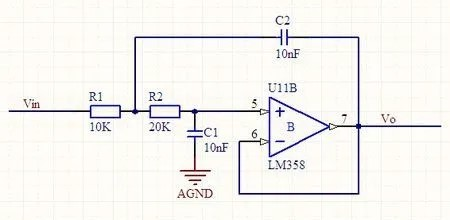
\includegraphics[width=0.8\linewidth]{fig/2.4.jpg}
		\caption{某示例电路图（低通滤波器？）}
		\label{fig:LPF}
	\end{figure}
	\paragraph{分析与结论}
	这里可以引用之前或之后的label，比如图~\ref{fig:LPF}或者表~\ref{tab:test}。
	\paragraph{三线表}
	\begin{table}[!htbp]
		\centering
		\caption{一个三线表示例}
		\label{tab:test}
		\begin{tabular}{lccc}
			\toprule
			test name & test value 1 & test value 2 & test value 3 \\
			\midrule
			name1 & v1 & v2 & v3 \\
			name2 & vv1 & vv2 & vv3 \\
			\bottomrule
		\end{tabular}
	\end{table}
	\subsubsection{硬件测试}
	\subsection{静态工作点设置}
	\section{实验小结及思考题}
	\setcounter{figure}{0}
	在切换section后，使用setcounter命令设置fig的编号，这样下面一张图才会是5.1而不是5.2。
	\begin{figure}[!htbp]
		\centering
		\includegraphics[width=0.8\linewidth]{fig/test-img.png}
		\caption{随便找的图}
		\label{fig:test}
	\end{figure}
	\begin{thebibliography}{99}
		\bibitem{Newton} Newton I, Hawking S, Biarnais F. Philosophiae Naturalis Principea Mathematica[C]//Annales de Chimie et de Physique. Royal Society Press, London, 1985, 431: 168-181.
		\bibitem{Einstein} Einstein A, Podolsky B, Rosen N. Can quantum-mechanical description of physical reality be considered complete?[J]. Physical review, 1935, 47(10): 777.
	\end{thebibliography}
	\appendix
	\section{实验原始数据记录} % 可选
	\section{实验过程照片} % 可选
	\section{实验代码} % 可选
\end{document}